\documentclass[tikz,border=10pt]{standalone}
\usetikzlibrary{arrows.meta, positioning, shapes.geometric, shapes.misc, fit, backgrounds, calc, matrix}

\tikzset{
    >=Latex,
    font=\sffamily\large,
    node distance=1.5cm and 3cm,
    dag_result/.style={
        rectangle, 
        draw=green!70!black, 
        fill=green!15, 
        very thick, 
        minimum width=4.5cm, 
        minimum height=1.5cm, 
        text width=5cm,
        align=center
    },
    dag_lemma/.style={
        rounded rectangle, 
        draw=orange!80!black, 
        fill=yellow!20, 
        very thick, 
        minimum width=4.5cm, 
        minimum height=1.5cm, 
        text width=5cm,
        align=center
    },
    dag_model/.style={
        ellipse, 
        draw=blue!70!black, 
        fill=blue!12, 
        very thick, 
        minimum width=4.5cm, 
        minimum height=1.5cm, 
        text width=4.5cm,
        align=center
    },
    dag_unformalized/.style={
        rectangle, 
        draw=gray!60!black, 
        fill=gray!10, 
        very thick, 
        dashed, 
        minimum width=4.5cm, 
        minimum height=1.5cm, 
        text width=5cm,
        align=center
    },
    dag_conditional/.style={
        rectangle, 
        rounded corners,
        draw=orange!80!black, 
        fill=orange!10, 
        very thick, 
        minimum width=4.5cm, 
        minimum height=1.5cm, 
        text width=5cm,
        align=center
    },
    dag_partial/.style={
        rectangle,
        rounded corners,
        draw=yellow!55!black,
        fill=yellow!10,
        very thick,
        dashed,
        minimum width=4.5cm,
        minimum height=1.5cm,
        text width=5cm,
        align=center
    },
    dag_scaffold/.style={
        rectangle,
        draw=gray!55!black,
        fill=white,
        very thick,
        dotted,
        minimum width=4.5cm,
        minimum height=1.5cm,
        text width=5cm,
        align=center
    },
    dag_caveat/.style={
        diamond, 
        draw=red!70!black, 
        fill=red!10, 
        minimum width=4cm, 
        align=center, 
        inner sep=0pt, 
        font=\sffamily\small
    },
    dag_arrow/.style={
        -{Stealth[scale=1.2]}, 
        very thick,
        shorten >=1.5pt,
        shorten <=1.5pt
    },
    dag_dashed_arrow/.style={
        -{Stealth[scale=1.2]}, 
        very thick, 
        dashed,
        shorten >=1.5pt,
        shorten <=1.5pt
    },
    dag_template_legend/.style={
        minimum width=2.6cm,
        minimum height=0.8cm,
        text width=2.45cm,
        inner sep=3pt,
        font=\sffamily\small,
        align=center
    },
    dag_template_note/.style={
        rectangle,
        draw=gray!50,
        fill=gray!5,
        rounded corners,
        text width=13cm,
        align=left,
        font=\sffamily\small,
        inner sep=6pt
    }
}

% Legend Helper
\newcommand{\daglegend}[2]{
    \node[draw, rounded corners, very thick, fit=#1, inner sep=12pt, label=above:\textbf{\Large Legend}] (#2) {};
}


\begin{document}
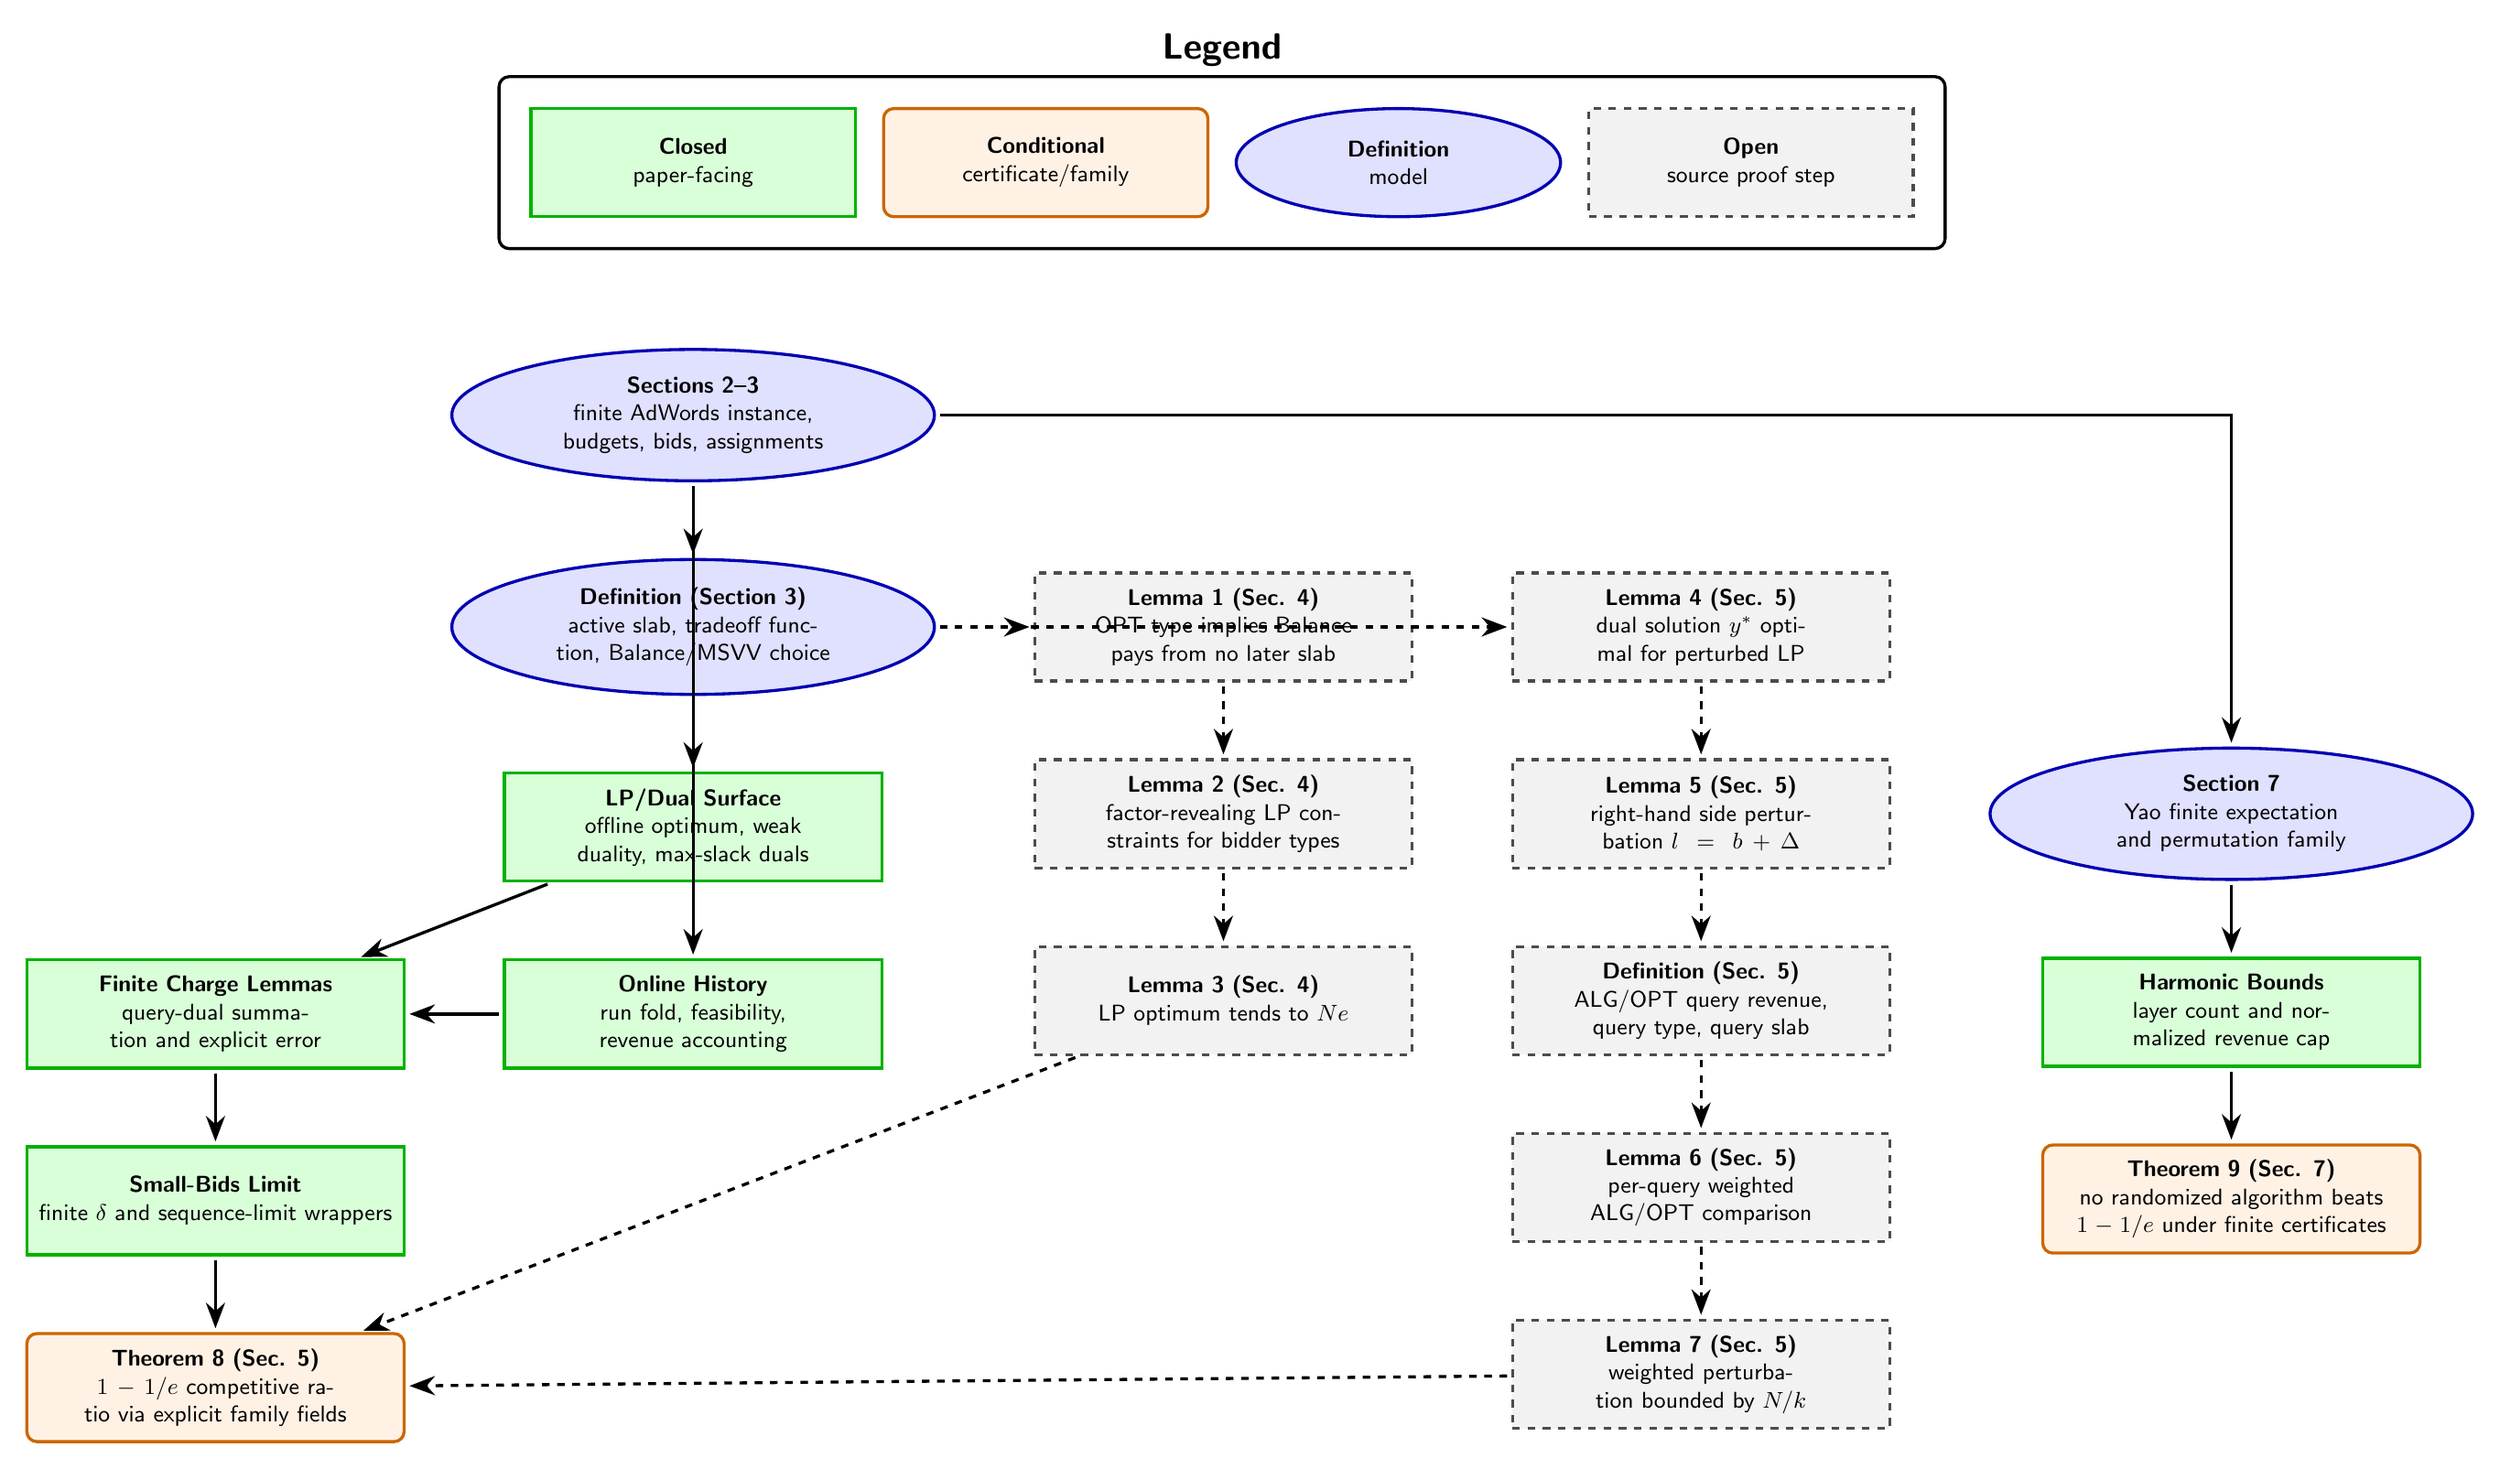
\begin{tikzpicture}[node distance=1.05cm and 1.35cm,
  every node/.style={font=\sffamily\small}]

% Legend
\node[dag_result, text width=2.9cm] (legRes) {\textbf{Closed}\\paper-facing};
\node[dag_conditional, right=0.35cm of legRes, text width=2.9cm] (legCond) {\textbf{Conditional}\\certificate/family};
\node[dag_model, right=0.35cm of legCond, text width=2.9cm] (legDef) {\textbf{Definition}\\model};
\node[dag_unformalized, right=0.35cm of legDef, text width=2.9cm] (legOpen) {\textbf{Open}\\source proof step};
\daglegend{(legRes)(legCond)(legDef)(legOpen)}{Legend}

% Model and algorithm surface
\node[dag_model, below=1.8cm of legRes] (AdWordsModel)
  {\textbf{Sections 2--3}\\finite AdWords instance, budgets, bids, assignments};
\node[dag_model, below=of AdWordsModel] (SlabDef)
  {\textbf{Definition (Section 3)}\\active slab, tradeoff function, Balance/MSVV choice};
\node[dag_result, below=of SlabDef] (LPDual)
  {\textbf{LP/Dual Surface}\\offline optimum, weak duality, max-slack duals};
\node[dag_result, below=of LPDual] (History)
  {\textbf{Online History}\\run fold, feasibility, revenue accounting};

% Source equal-bids factor-revealing LP path
\node[dag_unformalized, right=of SlabDef] (Lemma1)
  {\textbf{Lemma 1 (Sec. 4)}\\OPT type implies Balance pays from no later slab};
\node[dag_unformalized, below=of Lemma1] (Lemma2)
  {\textbf{Lemma 2 (Sec. 4)}\\factor-revealing LP constraints for bidder types};
\node[dag_unformalized, below=of Lemma2] (Lemma3)
  {\textbf{Lemma 3 (Sec. 4)}\\LP optimum tends to $Ne$};

% General-bids source path
\node[dag_unformalized, right=of Lemma1] (Lemma4)
  {\textbf{Lemma 4 (Sec. 5)}\\dual solution $y^*$ optimal for perturbed LP};
\node[dag_unformalized, below=of Lemma4] (Lemma5)
  {\textbf{Lemma 5 (Sec. 5)}\\right-hand side perturbation $l=b+\Delta$};
\node[dag_unformalized, below=of Lemma5] (QueryDef)
  {\textbf{Definition (Sec. 5)}\\ALG/OPT query revenue, query type, query slab};
\node[dag_unformalized, below=of QueryDef] (Lemma6)
  {\textbf{Lemma 6 (Sec. 5)}\\per-query weighted ALG/OPT comparison};
\node[dag_unformalized, below=of Lemma6] (Lemma7)
  {\textbf{Lemma 7 (Sec. 5)}\\weighted perturbation bounded by $N/k$};

% Lean route to theorem 8
\node[dag_result, left=of History] (Charge)
  {\textbf{Finite Charge Lemmas}\\query-dual summation and explicit error};
\node[dag_result, below=of Charge] (SmallBids)
  {\textbf{Small-Bids Limit}\\finite $\delta$ and sequence-limit wrappers};
\node[dag_conditional, below=of SmallBids] (Theorem8)
  {\textbf{Theorem 8 (Sec. 5)}\\$1-1/e$ competitive ratio via explicit family fields};

% Lower bound
\node[dag_model, right=of Lemma5] (Yao)
  {\textbf{Section 7}\\Yao finite expectation and permutation family};
\node[dag_result, below=of Yao] (Harmonic)
  {\textbf{Harmonic Bounds}\\layer count and normalized revenue cap};
\node[dag_conditional, below=of Harmonic] (Theorem9)
  {\textbf{Theorem 9 (Sec. 7)}\\no randomized algorithm beats $1-1/e$ under finite certificates};

% Edges
\draw[dag_arrow] (AdWordsModel) -- (SlabDef);
\draw[dag_arrow] (AdWordsModel) -- (LPDual);
\draw[dag_arrow] (AdWordsModel) -- (History);
\draw[dag_arrow] (LPDual) -- (Charge);
\draw[dag_arrow] (History) -- (Charge);
\draw[dag_arrow] (Charge) -- (SmallBids);
\draw[dag_arrow] (SmallBids) -- (Theorem8);

\draw[dag_dashed_arrow] (SlabDef) -- (Lemma1);
\draw[dag_dashed_arrow] (Lemma1) -- (Lemma2);
\draw[dag_dashed_arrow] (Lemma2) -- (Lemma3);
\draw[dag_dashed_arrow] (Lemma3) -- (Theorem8);
\draw[dag_dashed_arrow] (SlabDef) -- (Lemma4);
\draw[dag_dashed_arrow] (Lemma4) -- (Lemma5);
\draw[dag_dashed_arrow] (Lemma5) -- (QueryDef);
\draw[dag_dashed_arrow] (QueryDef) -- (Lemma6);
\draw[dag_dashed_arrow] (Lemma6) -- (Lemma7);
\draw[dag_dashed_arrow] (Lemma7) -- (Theorem8);

\draw[dag_arrow] (AdWordsModel.east) -| (Yao);
\draw[dag_arrow] (Yao) -- (Harmonic);
\draw[dag_arrow] (Harmonic) -- (Theorem9);

\end{tikzpicture}
\end{document}
